% ..............................................................................
% Demo of the fau-beamer template.
%
% Copyright 2022 by Tim Roith <tim.roith@fau.de>
%
% This program can be redistributed and/or modified under the terms
% of the GNU Public License, version 2.
%
% ------------------------------------------------------------------------------
\documentclass[final]{beamer}

% ========================================================================================
% Theme: inner, outer, font and colors
% ----------------------------------------------------------------------------------------
\usepackage[institute=Phil,
			%SecondLogo = template-art/FAUWortmarkeBlau.pdf,
			%ThirdLogo = template-art/FAUWortmarkeBlau.pdf,
			%WordMark=None,
			aspectratio=169,
			fontsize=11,
			fontbaselineskip=13,
			scale=1.,
			InsertTotalFoot
		   ]{styles/beamerthemefau}
% ----------------------------------------------------------------------------------------
% Input and output encoding
\usepackage[T1]{fontenc}
\usepackage[utf8]{inputenc}
% ----------------------------------------------------------------------------------------
% Language settings
\usepackage[english]{babel}

% ========================================================================================
% Fonts
% - Helvet is loaded by styles/beamerfonts
% - We use serif for math environements
% - isomath is used for upGreek letters
% ----------------------------------------------------------------------------------------
\usepackage{isomath}
\usefonttheme[onlymath]{serif}
\usepackage{exscale}
\usepackage{anyfontsize}
\setbeamercolor{alerted text}{fg=BaseColor}
% ----------------------------------------------------------------------------------------
% custom commands for symbols
\usepackage{styles/symbols}


% ========================================================================================
% Setup for Titlepage
% ----------------------------------------------------------------------------------------
\title[fau-beamer]{How Random is a Corpus?}
\subtitle{Topic 1.2.A Methodological issues and statistical analysis}
\author[X. Lu]{
Xinyao Lu\and%
Nathan Dykes\inst{1}
}
%
\institute[FAU]{%
\inst{1} Department of German Language and Literature, Chair of Computational Corpus Linguistics
}

% Instead of \institute you can also use the \thanks command
% ------------------------------------------------
%\author[T. Roith]{
%Tim Roith\thanks{Friedrich-Alexander Universität Erlangen-Nürnberg, Department Mathematik}\and%
%Second Author\thanks{Second Insitute}\and%
%Third Author\thanks{Third Insitute}%
%}

\date{12.07.24}


% ================================================
% Bibliography
% ------------------------------------------------
\usepackage{csquotes}
\usepackage[style=alphabetic, %alternatively: numeric, numeric-comp, and other from biblatex
			defernumbers=true,
			useprefix=true,%
			giveninits=true,%
			hyperref=true,%
			autocite=inline,%
			maxcitenames=5,%
			maxbibnames=20,%
			uniquename=init,%
			sortcites=true,% sort citations when multiple entries are passed to one cite command
			doi=true,%
			isbn=false,%
			url=false,%
			eprint=false,%
			backend=bibtex%
			]{biblatex}
\addbibresource{references.bib}
\setbeamertemplate{bibliography item}[text]


% ================================================
% Hyperref and setup
% ------------------------------------------------
\usepackage{hyperref}
\hypersetup{
	colorlinks = true,
	final=true, 
	plainpages=false,
	pdfstartview=FitV,
	pdftoolbar=true,
	pdfmenubar=true,
	pdfencoding=auto,
	psdextra,
	bookmarksopen=true,
	bookmarksnumbered=true,
	breaklinks=true,
	linktocpage=true,
	urlcolor=BaseColor,
	citecolor=BaseColor,
	linkcolor=BaseColor
}


% ================================================
% Additional packages
% ------------------------------------------------


% ================================================
% Various custom commands
% ------------------------------------------------
%\setbeameroption{show notes on second screen}
\begingroup\expandafter\expandafter\expandafter\endgroup
\expandafter\ifx\csname pdfsuppresswarningpagegroup\endcsname\relax
\else
  \pdfsuppresswarningpagegroup=1\relax
\fi
% Change color for cite locally
\newcommand{\colorcite}[3]{{\hypersetup{citecolor=#1}{\cite[#2]{#3}}}} 
% ------------------------------------------------
% ================================================
% The main document
% ------------------------------------------------
\begin{document}
% Title page
\begin{frame}[t,titleimage]{-}
\titlepage%
\end{frame}

% Stylized outline
%\begin{frame}[title]{-}
%	\tableofcontents
%\end{frame}


% input exmple sections
% ..............................................................................
% Demo of the fau-beamer template.
%
% Copyright 2022 by Tim Roith <tim.roith@fau.de>
%
% This program can be redistributed and/or modified under the terms
% of the GNU Public License, version 2.
%
% ------------------------------------------------------------------------------

% ------------------------------------------------------------------------------
\section{Topic Orientation}
% ..............................................................................
% Review
\subsection{Seminar Review}
\begin{frame}[t]{Seminar Review}{What did we learn in this seminar?}
	\begin{itemize}
		
		\item \textbf{Significance testing (Statistical methods)}
		\begin{itemize}
			\item Null hypothesis, p-value, chi-square test
		\end{itemize}
		\bigbreak
			
		\item \textbf{Corpus design}
		\begin{itemize}
			\item Social media corpora
			\item Spoken language corpora
		\end{itemize}
		\bigbreak
		
		\item \textbf{Application of  Corpus Linguistics (Results Interpretation)}
		\begin{itemize}
			\item Critical discourse analysis
			\item Translation studies
			\item Pragmatic studies
		\end{itemize}
		
	\end{itemize}
\end{frame}


% ..............................................................................
% Procedures
\subsection{Procedures of a Corpus Linguistics research}
\begin{frame}{Procedures of a Corpus Linguistics research}
	\begin{figure}
		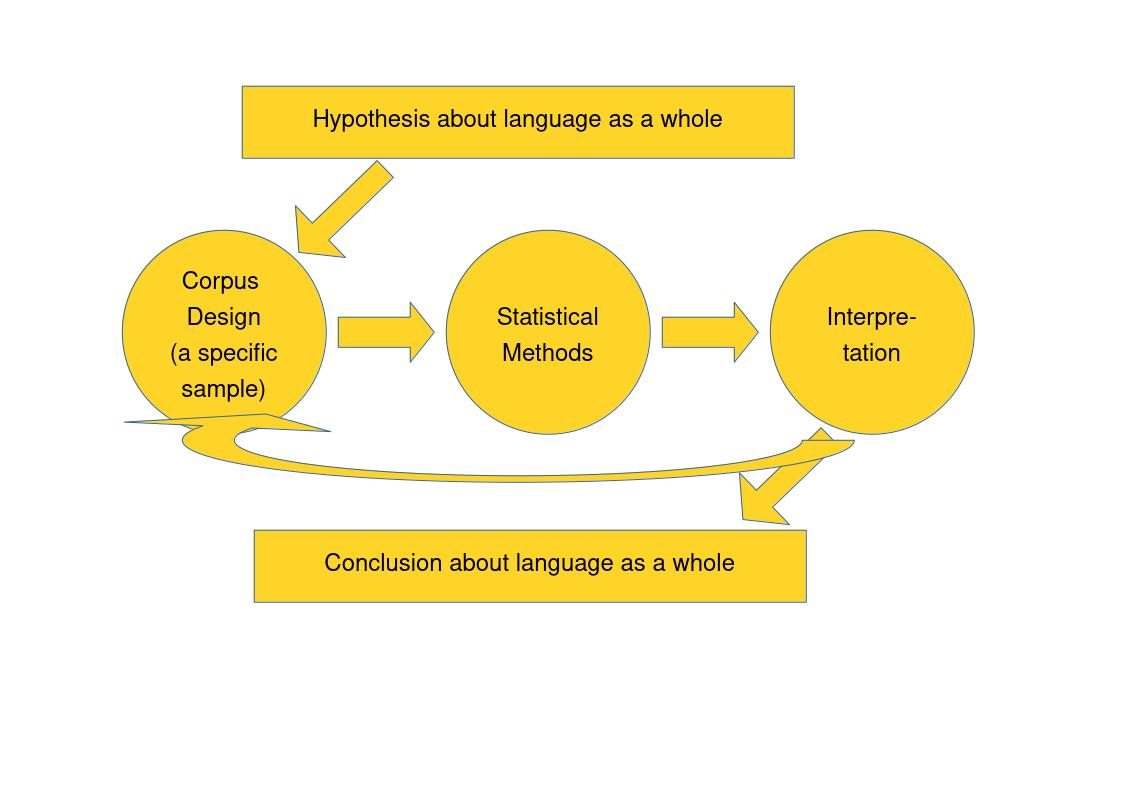
\includegraphics[width=.7\textwidth]{Figures/Procedures.jpg}
		\caption{Three steps in a typical CL research}
	\end{figure}
\end{frame}


% ..............................................................................
%Topic  key word
\subsection{Topic key word}
\begin{frame}[t]{Topic key word}{Evert: Reflection of Statistical Methods in Corpus Linguistics}
	
	\begin{itemize}
		\item \textit{why should we apply statistical methods (based on the \textbf{random sample} model) at all?} (in corpus linguistics)
		\begin{itemize}
			\item Evert, Stefan. "How Random is a Corpus? The Library Metaphor" Zeitschrift für Anglistik und Amerikanistik, vol. 54, no. 2, 2006, pp. 177-190.
		\end{itemize}
		\bigbreak
		\item What does \textbf{Randomness} actually mean in Corpus Linguistics?
		\bigbreak
		
		\item Sources of \textbf{(non-)Randomness}: Corpus design
		\bigbreak
		
		\item Validating the \textbf{(non-)Randomness}: Results interpretation 
	\end{itemize}
	
\end{frame}



% ..............................................................................
% Demo of the fau-beamer template.
%
% Copyright 2022 by Tim Roith <tim.roith@fau.de>
%
% This program can be redistributed and/or modified under the terms
% of the GNU Public License, version 2.
%
% ------------------------------------------------------------------------------

% ------------------------------------------------------------------------------
\section{Randomness and Non-Randomness}
% ..............................................................................
% Source of randomness
\subsection{Source of randomness}
\begin{frame}[t]{Source of randomness}{The library metapher}
	\begin{itemize}
		
		\item \textbf{A seeming conflict}
		\begin{itemize}
			\item \textit{statistical methods ... operate on random samples}
			\item \textit{very little (in language) is left to chance}
		\end{itemize}
		\bigbreak
			
		\item \textbf{The library metapher}
		\begin{itemize}
			\item \textit{... there is nothing random about the text in the library: every senetence was produced for some specific purpose.}
			\item \textit{The selection of a particular corpus} - \textit{picking an arbitrary book from one of the shelves}
			\item \textit{It is this choice which introduces an element of randomness into corpus frequency data.}
		\end{itemize}
		\bigbreak
		
		\item \textbf{Why randomness?}
		\begin{itemize}
			\item Statistical inference: Representativeness to (sub)language as a whole
		\end{itemize}
		
	\end{itemize}
\end{frame}

\begin{frame}{Source of randomness}{Illustrated in the procedures}
	\begin{figure}
		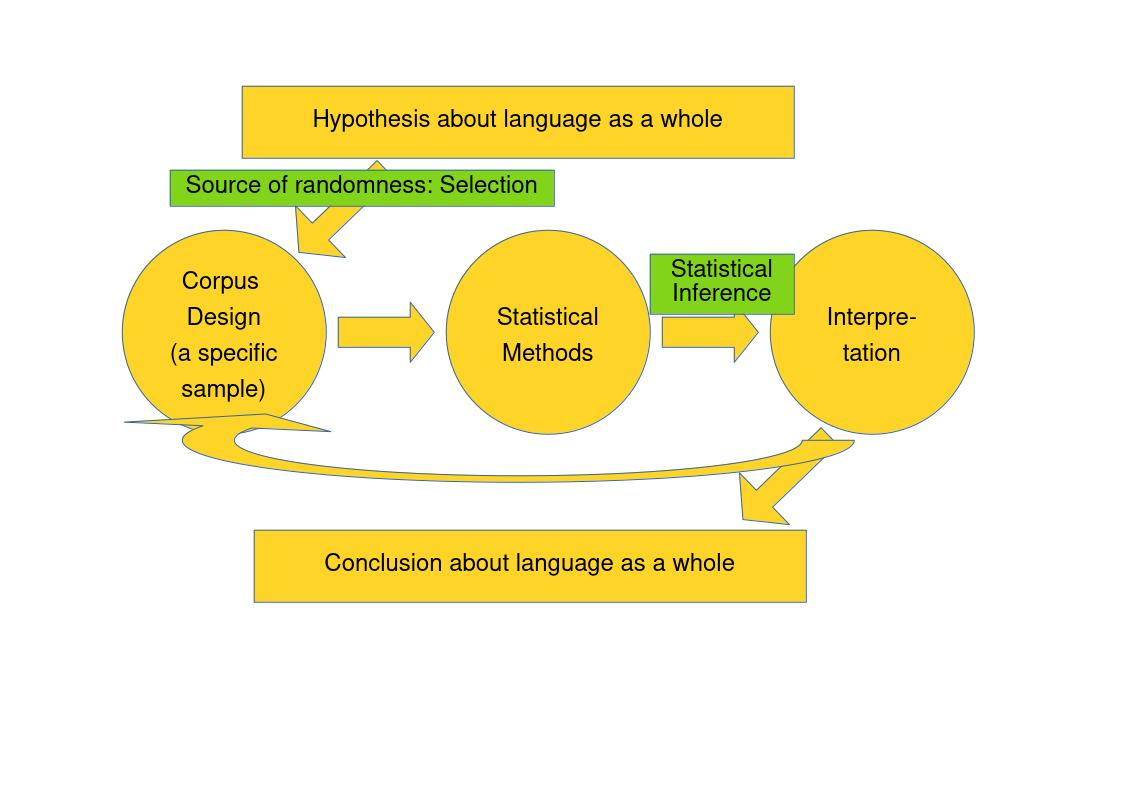
\includegraphics[width=.7\textwidth]{Figures/Randomness.jpg}
		\caption{Source of randomness}
	\end{figure}
\end{frame}


% Sources of non-randomness
\subsection{Sources of non-randomness}
\begin{frame}[t]{Sources of non-randomness}{Still not (completely) random?}
	
	\begin{itemize}
		\item \textbf{\textit{Balanced} samples}
		\begin{itemize}
			\item \textbf{External} source of non-randomness
			\item An issue of subjective language interpretation
		\end{itemize}
		\bigbreak
		
		\item \textbf{The unit of sampling} vs. \textbf{the unit of measurement}
		\begin{itemize}
			\item \textbf{Internal} source of non-randomness
			\item Clustering effect: \textit{a tendency to lump together}
			\item Language is NOT a bag of random words
		\end{itemize}
	\end{itemize}

\end{frame}

\begin{frame}{An evidence of internal non-randomness}{Underestimated variation}
	\begin{figure}
		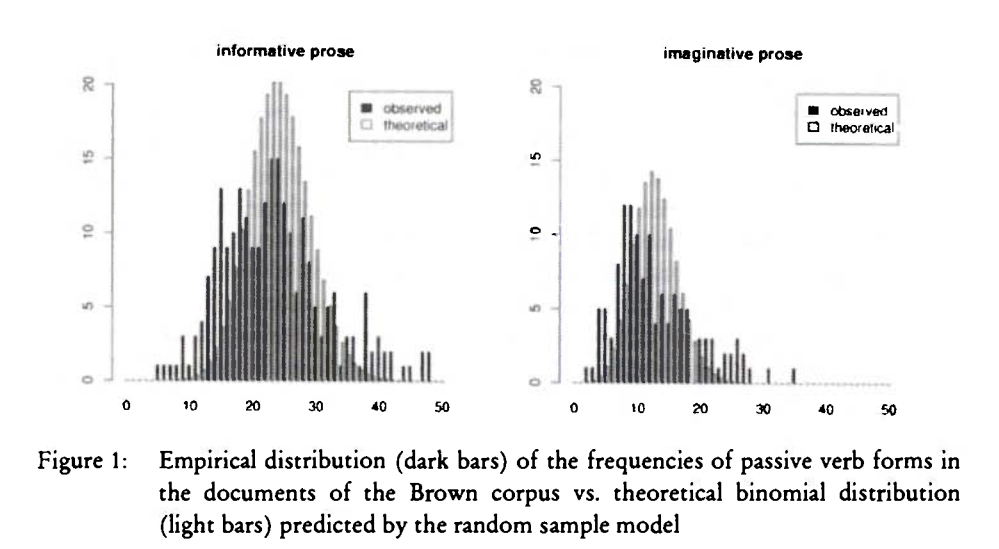
\includegraphics[width=.7\textwidth]{Figures/Distribution.png}
	\end{figure}
\end{frame}




% ..............................................................................
% Demo of the fau-beamer template.
%
% Copyright 2022 by Tim Roith <tim.roith@fau.de>
%
% This program can be redistributed and/or modified under the terms
% of the GNU Public License, version 2.
%
% ------------------------------------------------------------------------------

% ------------------------------------------------------------------------------
\section{Conclusion}
\begin{frame}[t]{Conclusion}{Things that statistics won't tell you.}
	\begin{itemize}
		
		\item \textbf{Statistical methods and corpus design}
		\begin{itemize}
			\item Statistics don't show the quality of corpus design.
			\item Conversely, the selection of texts provides the randomness (i. e. representativeness), which is the prerequisite of all statistical methods. 
		\end{itemize}
		\bigbreak
		
		\item \textbf{Statistical methods and interpretation}
		\begin{itemize}
			\item Two sources of randomness may reduce the validity of statistical reference: Imbalanced sampling and clustering effect.
			\item Real linguistic data usually have larger variation (an index of non-randomness) than theoretical expectation. 
		\end{itemize}
		
	\end{itemize}
\end{frame}



\begin{frame}{Thanks for your attention}{How does the elephant look like?}
	\begin{figure}
		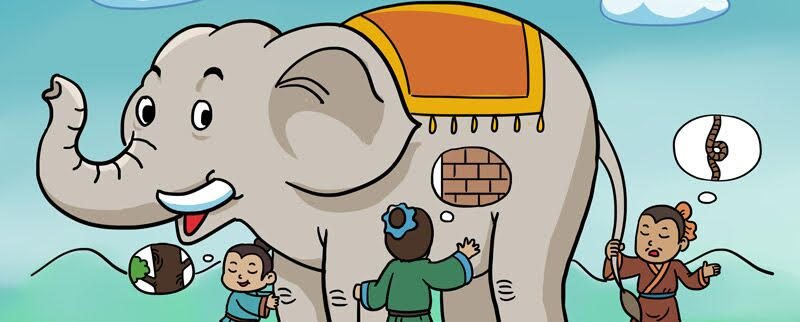
\includegraphics[width=.7\textwidth]{Figures/Elephant.jpg}
		\caption{Blind people touch an elephant}
	\end{figure}
\end{frame}

\begin{frame}[t]{References}
	%\nocite{stefanowitsch2020corpus}
	%\nocite{BaroniEvert}
	%\nocite{Evert}
	\nocite{*}
	\printbibliography[heading=none]
\end{frame}


\end{document}